% Asset ID: AS2MeasuresLocationSpreadTikZ-004
% Purpose: Show quartiles, IQR and optional outlier fences.
\documentclass[tikz,border=8pt]{standalone}
\usepackage{amsmath}
\usetikzlibrary{arrows.meta, positioning, decorations.pathreplacing}
\begin{document}
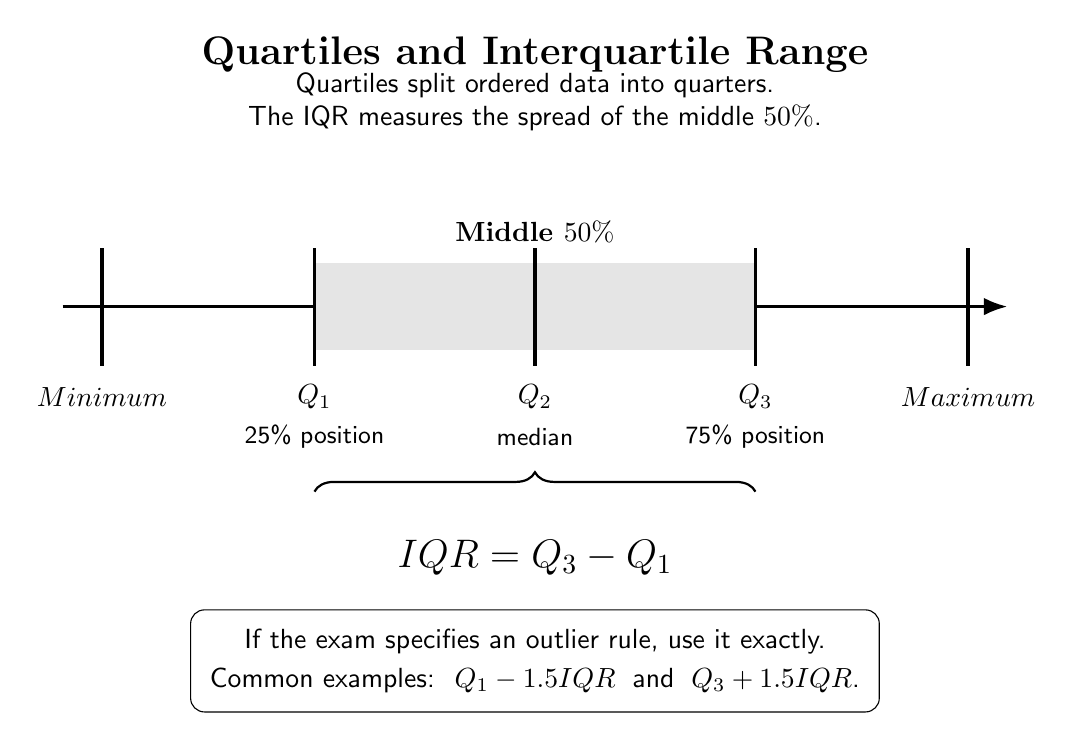
\begin{tikzpicture}[font=\sffamily, marker/.style={line width=1.2pt}, lab/.style={align=center, font=\small\sffamily}]
\node[font=\Large\bfseries] at (0,4.5) {Quartiles and Interquartile Range};
\node[align=center] at (0,3.9) {Quartiles split ordered data into quarters.\\The IQR measures the spread of the middle $50\%$.};
\draw[-{Latex[length=3mm]}, line width=1.1pt] (-6,1.3) -- (6,1.3);
\fill[gray!20] (-2.8,0.75) rectangle (2.8,1.85);
\foreach \x/\name/\desc in {-5.5/Minimum/, -2.8/Q_1/25\% position, 0/Q_2/median, 2.8/Q_3/75\% position, 5.5/Maximum/}{\draw[marker] (\x,0.55) -- (\x,2.05);\node[font=\bfseries] at (\x,0.15) {$\name$};\node[lab] at (\x,-0.35) {\desc};}
\node[font=\bfseries] at (0,2.25) {Middle $50\%$};
\draw[decorate, decoration={brace, amplitude=7pt}, thick] (-2.8,-1.05) -- (2.8,-1.05);
\node[below=5mm, font=\Large\bfseries] at (0,-1.05) {$IQR=Q_3-Q_1$};
\node[draw, rounded corners=5pt, align=center, inner sep=7pt] at (0,-3.2) {If the exam specifies an outlier rule, use it exactly.\\[2pt]Common examples: $\;Q_1-1.5IQR\;$ and $\;Q_3+1.5IQR$.};
\end{tikzpicture}
\end{document}
